\lab{Profiling Python Code}{Profiling}
\objective{Learn how to efficiently optimize Python code.}
\label{lab:ProfilingCode}

The best code goes through multiple drafts.
In a first draft, you should focus on writing code that does what is is supposed to and is easy to read.
After writing a fist draft, you may find that your code does not run as quickly as you need it to.
Then it is time to \emph{optimize} the most time consuming parts of your code so that they run as quickly as possible.

In this lab we will optimize the function \texttt{qr1()} that computes the QR decomposition of a matrix via the modified Gram-Schmidt algorithm (see Lab \ref{lab:QRdecomp}).
\begin{lstlisting}
import numpy as np
from scipy import linalg as la

def qr1(A):
    ncols = A.shape[1]
    Q = A.copy()
    R = np.zeros((ncols, ncols))
    for i in range(ncols):
        R[i, i] = la.norm(Q[:, i])
        Q[:, i] = Q[:, i]/la.norm(Q[:, i])
        for j in range(i+1, ncols):
            R[i, j] = Q[:, j].dot(Q[:, i])
            Q[:,j] = Q[:,j]-Q[:, j].dot(Q[:, i])*Q[:,i]
    return Q, R
\end{lstlisting}

\section*{What to optimize}
Python provides a \emph{profiler} that can identify where code spends most of its runtime.
The output of the profiler will tell you where to begin your optimization efforts.

In IPython\footnote{If you are not using IPython, you will need to use the \li{cProfile} module documented here: \url{https://docs.python.org/2/library/profile.html}.}, 
you can profile a function from the command line with \texttt{\%prun}.
Here we profile \texttt{qr1()} on a random $300 \times 300$ array.
\begin{lstlisting}
>>> A = np.random.rand(300, 300)
>>> \%prun qr1(A)
\end{lstlisting}

On this computer, we get the following output.

{\scriptsize
\begin{verbatim}
         97206 function calls in 1.343 seconds

   Ordered by: internal time

   ncalls  tottime  percall  cumtime  percall filename:lineno(function)
        1    0.998    0.998    1.342    1.342 profiling_hw.py:4(qr1)
    89700    0.319    0.000    0.319    0.000 {method 'dot' of 'numpy.ndarray' objects}
      600    0.006    0.000    0.012    0.000 function_base.py:526(asarray_chkfinite)
      600    0.006    0.000    0.009    0.000 linalg.py:1840(norm)
     1200    0.005    0.000    0.005    0.000 {method 'any' of 'numpy.ndarray' objects}
      600    0.002    0.000    0.002    0.000 {method 'reduce' of 'numpy.ufunc' objects}
     1200    0.001    0.000    0.001    0.000 {numpy.core.multiarray.array}
     1200    0.001    0.000    0.002    0.000 numeric.py:167(asarray)
        1    0.001    0.001    0.001    0.001 {method 'copy' of 'numpy.ndarray' objects}
      600    0.001    0.000    0.022    0.000 misc.py:7(norm)
      301    0.001    0.000    0.001    0.000 {range}
        1    0.001    0.001    0.001    0.001 {numpy.core.multiarray.zeros}
      600    0.001    0.000    0.001    0.000 {method 'ravel' of 'numpy.ndarray' objects}
      600    0.000    0.000    0.000    0.000 {method 'conj' of 'numpy.ndarray' objects}
        1    0.000    0.000    1.343    1.343 <string>:1(<module>)
        1    0.000    0.000    0.000    0.000 {method 'disable' of '_lsprof.Profiler' objects}
\end{verbatim}
}


The first line of the output tells us that executing \texttt{qr1(A)} results in almost 100,000 function calls.  
Then we see a table listing these functions along with data telling us how much time each takes.
Here, \texttt{ncalls} is the number of calls to the function, \texttt{tottime} is the total time spent in the function, and \texttt{cumtime} is the amount of time spent in the function including calls to other functions.

For example, the first line of the table is the function \texttt{qr1(A)} itself. 
This function was called once, it took 1.342s to run, and 0.344s of that was spent in calls to other functions.
Of that 0.344s, there were 0.319s spent on 89,700 calls to \texttt{np.dot()}.

With this output, we see that most time is spent in multiplying matrices.
Since we cannot write a faster method to do this multiplication, we may want to try to reduce the number of matrix multiplications we perform.



\section*{How to Optimize}
Once you have identified those parts of your code that take the most time, how do you make them run faster?
This section lists a few ideas.
Always, you should use the profiling and timing functions to help you decide when an optimization is actually useful.

\subsection*{Avoid recomputing values}
In our function \texttt{qr1()}, we can avoid recomputing \texttt{R[i,i]} in the outer loop and \texttt{R[i,j]} in the inner loop.
The rewritten function is as follows:
\begin{lstlisting}
def qr2(A):
    ncols = A.shape[1]
    Q = A.copy()
    R = np.zeros((ncols, ncols))
    for i in range(ncols):
        R[i, i] = la.norm(Q[:, i])
        Q[:, i] = Q[:, i]/R[i, i]
        for j in range(i+1, ncols):
            R[i, j] = Q[:, j].dot(Q[:, i])
            Q[:,j] = Q[:,j]-R[i, j]*Q[:,i]
    return Q, R
\end{lstlisting}

Profiling \texttt{qr2()} on a $300 \times 300$ matrix produces the following output.

{\scriptsize
\begin{verbatim}
         48756 function calls in 1.047 seconds

   Ordered by: internal time

   ncalls  tottime  percall  cumtime  percall filename:lineno(function)
        1    0.863    0.863    1.047    1.047 profiling_hw.py:16(qr2)
    44850    0.171    0.000    0.171    0.000 {method 'dot' of 'numpy.ndarray' objects}
      300    0.003    0.000    0.006    0.000 function_base.py:526(asarray_chkfinite)
      300    0.003    0.000    0.005    0.000 linalg.py:1840(norm)
      600    0.002    0.000    0.002    0.000 {method 'any' of 'numpy.ndarray' objects}
      300    0.001    0.000    0.001    0.000 {method 'reduce' of 'numpy.ufunc' objects}
      301    0.001    0.000    0.001    0.000 {range}
      600    0.001    0.000    0.001    0.000 {numpy.core.multiarray.array}
      600    0.001    0.000    0.001    0.000 numeric.py:167(asarray)
      300    0.000    0.000    0.012    0.000 misc.py:7(norm)
        1    0.000    0.000    0.000    0.000 {method 'copy' of 'numpy.ndarray' objects}
      300    0.000    0.000    0.000    0.000 {method 'ravel' of 'numpy.ndarray' objects}
        1    0.000    0.000    1.047    1.047 <string>:1(<module>)
      300    0.000    0.000    0.000    0.000 {method 'conj' of 'numpy.ndarray' objects}
        1    0.000    0.000    0.000    0.000 {numpy.core.multiarray.zeros}
        1    0.000    0.000    0.000    0.000 {method 'disable' of '_lsprof.Profiler' objects}
\end{verbatim}
}

Our optimization reduced almost every kind of function call by half, and reduced the total run time by 0.295s.

Some less obvious ways to eliminate excess computations include moving computations out of loops, not copying large data structures, and simplifying mathematical expressions.


\subsection*{Avoid nested loops}
The best way to do this is to use NumPy array operations instead of iterating through arrays.
If you must use nested loops, focus your optimization efforts on the innermost loop, which gets called the most times.

\subsection*{Use existing functions instead of writing your own}
If there is an intuitive operation you would like to perform on an array, chances are that NumPy or another library already has a function that does it.
Python and NumPy functions have already been optimized, and are usually many times faster than the equivalent you might write.
We saw an example of this in Lab \ref{} where we compared NumPy array multiplication with our own matrix multiplication implemented in Python.

\subsection*{Use generators when possible}
When you are iterating through a list, you can often replace the list with a \emph{generator}.
Instead of storing the entire list in memory, a generator computes each item as it is needed. 
For example, the code
\begin{lstlisting}
>>> for i in range(100):
>>>     print i
\end{lstlisting}
stores the numbers 0 to 99 in memory, looks up each one in turn, and prints it. 
On the other hand, the code
\begin{lstlisting}
>>> for i in xrange(100):
>>>     print i
\end{lstlisting}
uses a generator instead of a list. 
This code computes the first number in the specified range (which is 0), and prints it.
Then it computes the next number (which is 1) and prints that.

It is also possible to write your own generators. 
See \url{https://docs.python.org/2/tutorial/classes.html#generators} and \url{https://wiki.python.org/moin/Generators} for more information.

In our example, replacing each \texttt{range} with \texttt{xrange} does not speed up \texttt{qr2()} by a noticeable amount.

\subsection*{Avoid excessive function calls}
Function calls take time.
Moreover, looking up methods associated with objects takes time.
Removing ``dots'' can significantly speed up execution time.

For example, we could rewrite our function to reduce the number of times we need to look up the function \texttt{la.norm()}.

\begin{lstlisting}
def qr2(A):
    norm = la.norm
    ncols = A.shape[1]
    Q = A.copy()
    R = np.zeros((ncols, ncols))
    for i in range(ncols):
        R[i, i] = norm(Q[:, i])
        Q[:, i] = Q[:, i]/R[i, i]
        for j in range(i+1, ncols):
            R[i, j] = Q[:, j].dot(Q[:, i])
            Q[:,j] = Q[:,j]-R[i, j]*Q[:,i]
    return Q, R
\end{lstlisting}
Once again, an analysis with \texttt{\%prun} reveals that this optimization does not help significantly in this case.


\subsection*{Write Pythonic code}
Several special features of Python allow you to write fast code easily.
First, list comprehensions are much faster than for loops.
For example, replace
\begin{lstlisting}
>>> mylist = []
>>> for i in xrange(100):
>>>     mylist.append(math.sqrt(i))
\end{lstlisting}
with 
\begin{lstlisting}
>>> mylist = [math.sqrt(i) for i in xrange(100)]
\end{lstlisting}
When it can be used, the function \texttt{map()} is even faster.
\begin{lstlisting}
>>> mylist = map(math.sqrt, xrange(100))
\end{lstlisting}
The analog of a list comprehension also exists for generators, dictionaries, and sets.

Second, swap values with a single assignment.
\begin{lstlisting}
>>> a, b = 1, 2
>>> a, b = b, a
>>> print a, b
2 1
\end{lstlisting}

Third, many non-Boolean objects in Python have truth values.
For example, numbers are \texttt{False} when equal to zero and \texttt{True} otherwise.
Similarly, lists and strings are \texttt{False} when they are empty and \texttt{True} otherwise.
So when \texttt{a} is a number, instead of
\begin{lstlisting}
>>> if a != 0:
\end{lstlisting}
use
\begin{lstlisting}
>>> if a:
\end{lstlisting}
\subsection*{Use Cython}
We will discuss Cython at the end of this lab.

\subsection*{Use a more efficient algorithm}
The optimizations discussed thus far will speed up your code at most by a constant.
They will not change the complexity of your code.
In order to reduce the complexity (say from $O(n^2)$ to $O(n \log(n))$), you typically need to change your algorithm.









\section*{When to Stop}
You don't need to apply every possible optimization to your code.
When your code runs acceptably fast, stop optimizing.



\section*{Cython}
Cython code is basically Python with extra type declarations.
This code is then compiled into C, which---depending on the details---can run much faster than the Python equivalent.
In this lab we will introduce Cython as a language and discuss how it can be used to speed up Python code.

\subsection*{Compiling Cython}
With a few exceptions, every Python program is also a Cython program.
For example, suppose you save the following script as \texttt{cymodule.pyx}.
\begin{lstlisting}
import numpy as np
from scipy import linalg as la

def qr(A):
    norm = la.norm
    ncols = A.shape[1]
    Q = A.copy()
    R = np.zeros((ncols, ncols))
    for i in range(ncols):
        R[i, i] = norm(Q[:, i])
        Q[:, i] = Q[:, i]/R[i, i]
        for j in range(i+1, ncols):
            R[i, j] = Q[:, j].dot(Q[:, i])
            Q[:,j] = Q[:,j]-R[i, j]*Q[:,i]
    return Q, R
\end{lstlisting}
To compile this code as Cython, we need to write another script, call it \texttt{setup.py}.
\lstinputlisting[style=fromfile, language=Python]{setup.py}
To run the setup script, type the following in the command line.
\footnote{Note that \texttt{python} in this line will need to refer to your version of Python that comes with Cython. 
Often, you will need to replace \texttt{python} with a path pointing to a specific distribution of Python.}
\begin{lstlisting}
>>> python setup.py build_ext --inplace
\end{lstlisting}
Now start up IPython in the same directory where you ran the setup script.
You can import \texttt{cymodule} just as if it were a Python module.
\begin{lstlisting}
>>> import cymodule
>>> cymodule.qr(A)
\end{lstlisting}

\subsection*{Speeding up Cython with type declarations}
So far, our Cythonized \texttt{qr()} function does not run any faster than the Python version.
\footnote{Sometimes you will see speedup immediately after Cythonizing a Python function.}
The simplest way to take advantage of the C-compilation is to declare data types, as you would in a C program.
All Cython data types and their NumPy equivalents are listed in Table \ref{table:cython_types}.

\begin{table}
\begin{center}
\begin{tabular}{|p{2.8cm}|p{2.5cm}|p{6cm}|}
\hline
Cython Type & NumPy Type& Description \\
\hline
float & float32 & 32 bit floating point number \\
double & float64 & 64 bit floating point number \\
float complex & complex64 & 64 bit floating point complex number \\
double complex & complex128 & 128 bit floating point complex number \\
char & int8 & 8 bit signed integer \\
unsigned char & uint8 & 8 bit unsigned integer \\
short & int16 & 16 bit signed integer \\
unsigned short & uint16 & 16 bit unsigned integer \\
int & int32 & 32 bit signed integer \\
unsigned int & uint32 & 32 bit unsigned integer \\
long & int32 or int64 & 32 or 64 bit signed integer (depends on platform) \\
unsigned long & uint32 or uint64 & 32 or 64 bit unsigned integer (depends on platform ) \\
long long & int64 & 64 bit signed integer \\
unsigned long long & uint64 & 64 bit unsigned integer \\
\hline
\end{tabular}
\end{center}
\caption{Numeric types available in Cython.}
\label{table:cython_types}
\end{table}

In our example, when we declare the index \texttt{j} to be an \texttt{int}, the inner for loop is pushed into C (instead of Python), speeding up our code immensely.
We do this by modifying \texttt{cymodule.pyx} as follows.
\begin{lstlisting}
...
def qr():
    cdef int j
    ncols = A.shape[1]
    Q = A.copy()
    ...
\end{lstlisting}

We could also declare \texttt{i} to be an int, but the effect of doing so is negligible.

After modifying \texttt{cymodule.pyx}, we must recompile it by running the script \texttt{setup.py}, and then re-import it into Python.
When we profile this function, we see that it is indeed a good deal faster than its Python cousin, and all the speed up is in the function itself (where the for loops are).
{\scriptsize
\begin{verbatim}
   ...
   ncalls  tottime  percall  cumtime  percall filename:lineno(function)
        1    0.949    0.949    0.961    0.961 {cymodule.qr}
   ...
       \end{verbatim}
       }
Similarly, you can speed up function calls in Cython by declaring the types of some or all of the arguments.
\begin{lstlisting}
def myfunction(double arg1, int arg2, arg3):
    ...
\end{lstlisting}


\subsection*{A caution}
NumPy's array methods are usually faster than a Cython equivalent you could code yourself.
If you are unsure which method is fastest, time them.

Moreover, a good algorithm written with a slow language (like Python) is faster than a bad algorithm written in a fast language (like C).
Hence, focus on writing fast algorithms with good Python code, and only use Cython when and where it is necessary.





\begin{problem}
Practice profiling and optimizing functions you have already written.
Some suggested functions are listed below.
\begin{itemize}
\item LU decomposition (Lab \ref{lab:ChangeBasis}). 
\item Householder triangularization or Hessenburg decomposition (Lab \ref{lab:QRdecomp}).
\item Givens triangularization (Lab \ref{lab:givens})
\item Image Segmentation (Lab \ref{lab:ImgSeg_eigenvalues})
\item Eigenvalue Solvers (Lab \ref{lab:EigSolve})
\end{itemize}
Your solution should include a before and after profiling of the function.  
It should also include a list of changes, the reasoning behind the changes, and the effect of the changes on runtime.  

It is possible that you will not be able to speed up the function significantly. 
Remember it is more important for code to be readable than to execute quickly.
\end{problem}




















      
\section*{More on Cython (Optional)}
This section has a more complete introduction to Cython. 
For another reference, see \url{http://docs.cython.org/src/tutorial/cython_tutorial.html}.

\subsection*{Compilation}

Cython code is usually written in a \texttt{.pyx} file, which is then compiled to C.
Next the C is compiled to a Python extension written in machine code.
Figure \ref{cython:compilation} shows how Cython code is compiled and called.

\begin{figure}
\centering
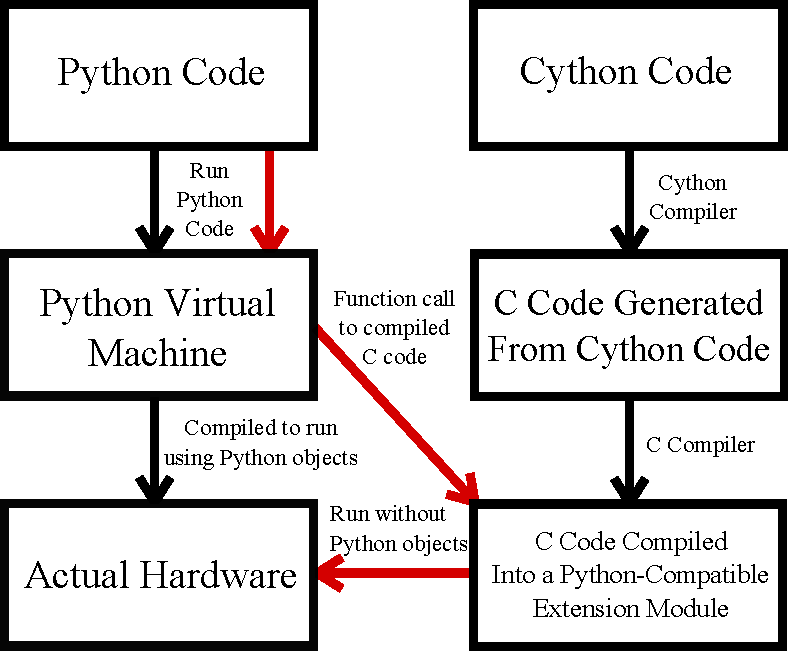
\includegraphics[width=.7\textwidth]{compilation.pdf}
\caption{A diagram showing how Cython code is compiled and called.
The path from calling a Cython function in a Python file to its evaluation is shown in red.}
\label{cython:compilation}
\end{figure}

These two compilations (first to C and then to a Python extension) are accomplished by the script \texttt{setup.py} discussed earlier in this lab.
\lstinputlisting[style=fromfile, language=Python]{setup.py}
The call to \texttt{cythonize()} compiles \texttt{cymodule.pyx} to C, and the call to \texttt{setup()} converts the C code to a Python extension.

\begin{info}
You can learn more about the Python/C balance in your Cython file with the following line.
\begin{lstlisting}
>>> cython -a cymodule.pyx
\end{lstlisting}
This will generate a \li{html} file that you can open with your web browser.
It will show the lines that use Python in bright yellow and lines that use C in white.
\end{info}

Cython code can be compiled and imported to IPython with the Cython magic function.
Load this function with the following command.
\footnote{In older versions of IPython and Cython, you may need to use the command \li{\%load_ext cythonmagic}.}
\begin{lstlisting}
>>> \%load_ext Cython
\end{lstlisting}
Now you can define any Cython function in the command line by prefacing it with \li{\%\%cython}.
\begin{lstlisting}
>>> \%\%cython
>>> import numpy as np
>>> from scipy import linalg as la
>>> def qr():
>>>     cdef int j
>>> ...
\end{lstlisting}

\subsection*{Type Declarations}
Type declarations make Cython faster than Python because a computer can process numbers faster when it knows ahead of time what type they are.
Declaring a variable type in Cython makes the variable a native machine type instead of a Python object.

You can initialize a variable when it is declared or afterwards.
It is possible to initialize several variables at once, as demonstrated below.

\begin{lstlisting}
# Declare integer variables i, j, and k.
# Set k equal to 2.
cdef int i, j, k=2

cdef:
    # Declare and initialize m equal to 4 and n equal to 5.
    int m=4, n=5
    # Declare and initialize e equal to 2.71.
    double e = 2.71
    # Declare a double precision complex number a.
    double complex a
\end{lstlisting}

\begin{warn}
Unlike Python integers, which can be arbitrarily large, Cython integers can overflow.
\end{warn} 

\subsection*{Arrays in Cython}
You can also declare types for arrays.
Doing so produces a \emph{typed memoryview}, or Cython array.
As with ordinary variables, typed memoryviews can be initialized when they are declared or later.
\begin{lstlisting}
# Define a NumPy array
A = np.linspace(0,1,6)

# Create typed memoryviews on A and B
cdef double[:] cA = A
cdef int[:,:] cB

# Initialize cB
cB = np.array([[1,2],[3,4],[5,6]], dtype=np.dtype("i"))
\end{lstlisting}

Accessing single entries from a memoryview is faster than accessing entries of a NumPy array.
Also, passing slices of a memoryview to a Cython function is fast.
However, memoryviews do not support mathematical operations.
These must be performed on NumPy objects, or by looping through the arrays.

\begin{info}
Memoryviews can be passed as arguments to most NumPy functions.
Numpy includes functions for all common arithmetic operations.
For example, you can add typed memoryviews with \li{c = np.add(a, b)}.
This may or may not be faster than looping through the array.
\end{info}

\subsection*{Compiler Directives}
When you access elements of an array, Cython checks that the indices are within bounds.
Cython also allows negative indexing the same way Python does.
These features slow down code execution.
After a program has been carefully debugged, they may be removed via \emph{compiler directives}.

Compiler directives in Cython can be included as comments or function decorators.
Directives included in comments will apply to the whole file, while function decorators will only apply to the function immediately following.
The comments to turn off bounds checking and negative indices are
\begin{lstlisting}
# cython: boundscheck=False
# cython: wraparound=False
\end{lstlisting}
To use the function decorators, first import the \li{cython} module by including the line \li{cimport cython} in your import statements.
The decorators are
\begin{lstlisting}
cimport cython
@cython.boundscheck(False)
@cython.wraparound(False)
\end{lstlisting}

Cython has many other compiler directives, including \li{cdivision}.
When \li{cdivision} is set to \li{True}, the \li{\%} operator returns a number with the sign of the first argument (like in C).
Also, division by 0 will no longer raise a \li{ZeroDivisionError}, which will increase the speed of your program.

\subsection*{More on functions in Cython}
Speed up function calls in Cython by declaring the types of some or all of the arguments.
\begin{lstlisting}
def myfunction(double[:] X, int n, double h, items):
    ...
\end{lstlisting}
If we pass in a NumPy array for the argument \li{X}, Cython will convert it to a typed memoryview before it enters the function.
However, if we pass in a NumPy array for \li{items}, it will remain a NumPy array in the function.
Both typed and untyped arguments can be made into keyword arguments.

Cython also allows you to make C functions that are only callable within the C extension you are currently building.
They are not ported into the Python namespace.
These functions are declared using the same syntax as in Python, except the keyword \li{def} is replaced with \li{cdef}.
The keyword \li{cpdef} combines \li{def} and \li{cdef} by creasting two versions of the function: one for Python and one for C.

You can also specify the return type for functions declared using \li{cdef} and \li{cpdef}, as in the code below.
\begin{lstlisting}
cpdef int myfunction(double[:] X, int n, double h, items):
    ...
\end{lstlisting}

\subsection*{Some examples}
The following Python function computes the dot product of two 1-D arrays.
\begin{lstlisting}
def pydot(A, B):
    tot = 0.
    for i in xrange(A.shape[0]):
        tot += A[i] * B[i]
    return tot
\end{lstlisting}
A C equivalent can be compiled from the following Cython code.
\begin{lstlisting}
cimport cython

@cython.boundscheck(False)
@cython.wraparound(False)
def cydot(double[:] A, double[:] B):
    cdef double tot=0.
    cdef int i
    for i in xrange(A.shape[0]):
        tot += A[i] * B[i]
    return tot
\end{lstlisting}

Figure \ref{cython:dot} compares the speed of \li{pydot()}, \li{cydot()}, and the \li{dot()} method of a NumPy array.

\begin{figure}
\centering
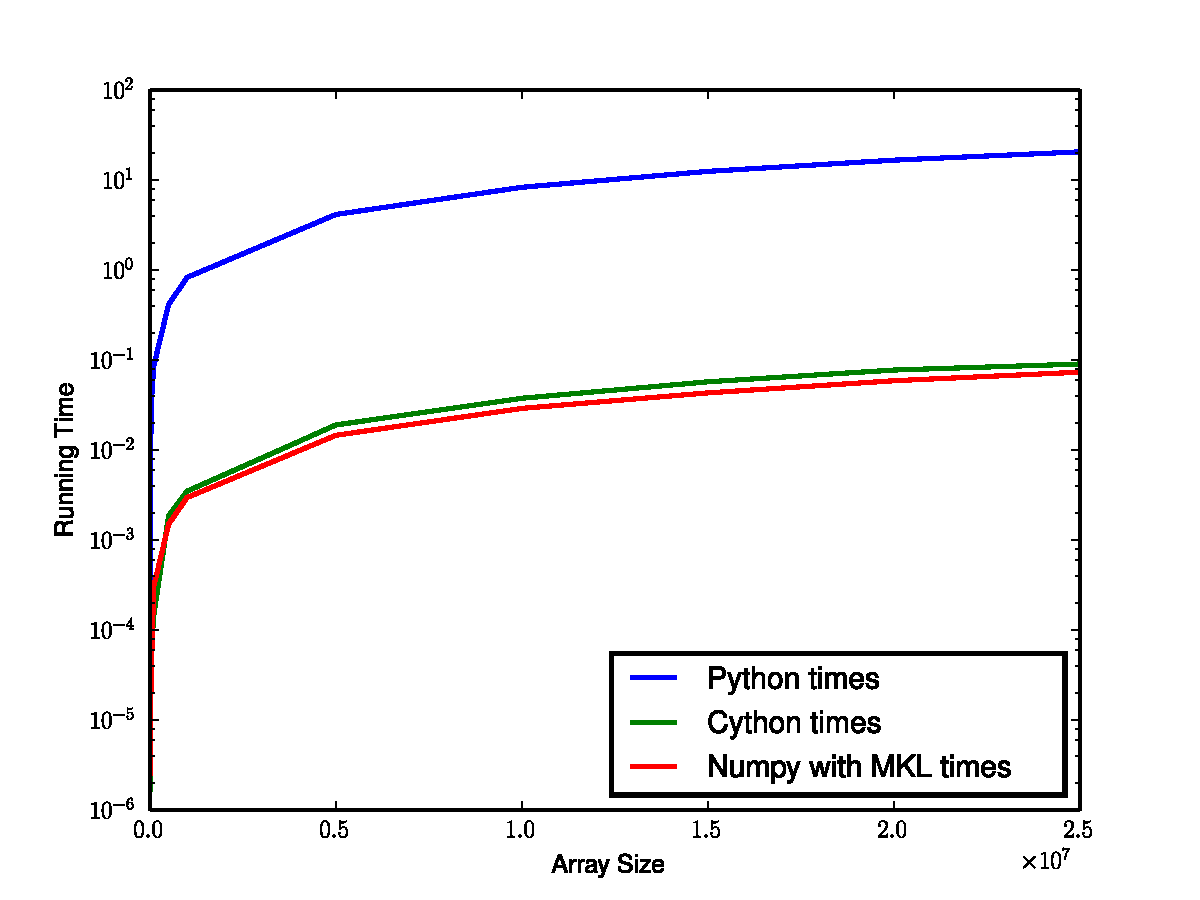
\includegraphics[width=\textwidth]{dot.pdf}
\caption{The running times of\li{pydot()}, \li{cydot()}, and the \li{dot()} method of a NumPy array on vectors of length ``Array Size.''
The Cython version runs almost as fast as the version built into NumPy.}
\label{cython:dot}
\end{figure}

For a second example, we will write functions which compute $AA^T$ from $A$.
That is, given \li{A}, these functions compute \li{B} where
\li{B[i,j] = dot(A[i],A[j])}.

Here is the Python solution.
\begin{lstlisting}
def pyrowdot(A):
    B = np.empty((A.shape[0], A.shape[0]))
    for i in xrange(A.shape[0]):
        for j in xrange(i):
            B[i,j] = pydot(A[i], A[j])
        B[i,i] = pydot(A[i], A[i])
    for i in xrange(A.shape[0]):
        for j in xrange(i+1, A.shape[0]):
            B[i,j] = B[j,i]
    return B
\end{lstlisting}

Here is the Cython solution. 
We changed the function \li{cydot()} to a C function since it will only be called by \li{cyrowdot()}.
Also, the Cython solution uses a typed memoryview of its input.

\begin{lstlisting}
import numpy as np
cimport cython
# cython: boundscheck=False
# cython: wraparound=False

cdef double cydot(double[:] A, double[:] B):
    cdef double tot=0.
    cdef int i, n=A.shape[0]
    for i in xrange(n):
        tot += A[i] * B[i]
    return tot

def cyrowdot(double[:,:] A):
    cdef double[:,:] B = np.empty((A.shape[0], A.shape[0]))
    cdef int i, j, n=A.shape[0]
    for i in xrange(n):
        for j in xrange(i):
           B[i,j] = cydot(A[i], A[j])
        B[i,i] = cydot(A[i], A[i])
    for i in xrange(n):
        for j in xrange(i+1, n):
            B[i,j] = B[j,i]
    return np.array(B)
\end{lstlisting}

This can also be done in NumPy by running \li{A.dot(A.T)}.
The timings of \li{pyrowdot()}, \li{cyrowdot()}, and the NumPy command \li{A.dot(A.T)} are shown in Figure \ref{cython:rowdot}.

\begin{figure}
\centering
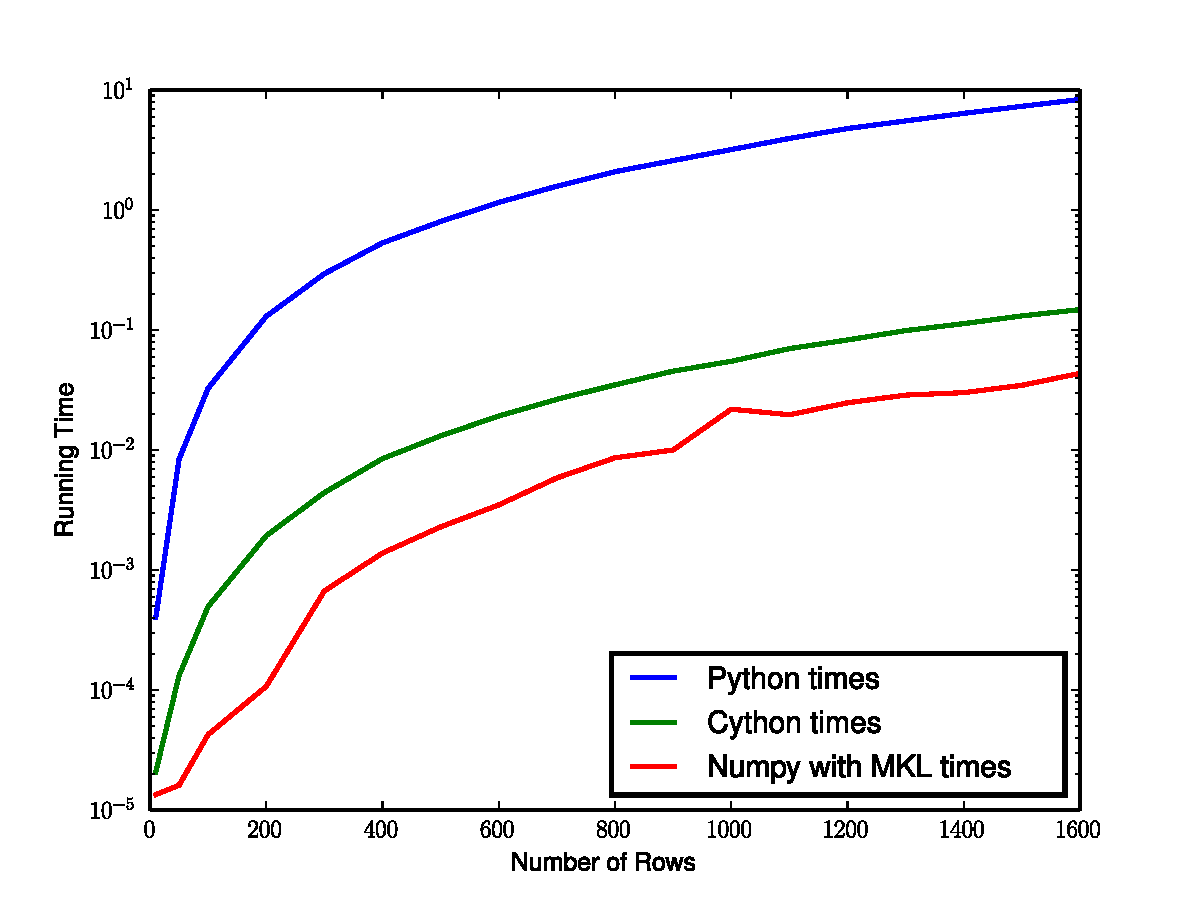
\includegraphics[width=\textwidth]{rowdot.pdf}
\caption{The timings of \li{pyrowdot()}, \li{cyrowdot()}, and the NumPy command \li{A.dot(A.T)}.
The arrays used for testing were $n\times 3$ where $n$ is shown along the horizontal axis.}
\label{cython:rowdot}
\end{figure}

In both of these examples, NumPy's implementation was faster than the version we wrote in Cython.

\begin{problem}
\leavevmode
\begin{enumerate}
\item Write the following function in Python.
\begin{lstlisting}
def pysum(X):
    ''' Return the sum of the elements of X.
    
    INPUTS:
    X - a 1-D NumPy array
    ''''
\end{lstlisting}

\item Rewrite the same function in Cython using a typed for-loop, a typed memoryview of \li{X}, and appropriate compiler directives.

\item Compare the speed of the functions you just wrote, the builtin \li{sum()} function, and NumPy's \li{sum()} function.
\end{enumerate}
\end{problem}

\begin{problem}
The code below defines a Python function which takes a matrix to the $n$th power.
\begin{lstlisting}
def pymatpow(X, power):
    ''' Return X^{power}.
    
    INPUTS:
    X		- A square 2-D NumPy array
    power	- An integer
    '''
    prod = X.copy()
    temparr = np.empty_like(X[0])
    size = X.shape[0]
    for n in xrange(1, power):
        for i in xrange(size):
            for j in xrange(size):
                tot = 0.
                for k in xrange(size):
                    tot += prod[i,k] * X[k,j]
                temparr[j] = tot
            prod[i] = temparr
    return prod
\end{lstlisting}

\begin{enumerate}
\item Port \li{pymatpow()} to Cython using typed for-loops, typed arrays, and appropriate compiler directives.
\item Compare the speed of \li{pymatpow()}, the function you just wrote, and the \li{np.dot()} function.
\end{enumerate}
NumPy takes products of matrices by calling BLAS and LAPACK, which are heavily optimized linear algebra libraries written in C, assembly, and Fortran.
\end{problem}


\begin{problem}
In Lab \ref{lab:ChangeBasis} you wrote a function to compute the LU decomposition of a matrix.
\begin{enumerate}
\item Rewrite this function so it performs every operation element-by-element instead of using NumPy array operations.
\item Port the function from part (a) to Cython.
Use typed for-loops, typed memoryviews, and appropriate compiler directives.
You may assume that you are only dealing with real arrays of double precision floating point numbers.
\item Compare the speed of your new solutions to the speed of the NumPy version you wrote earlier.
\end{enumerate}
\end{problem}


The correct choice of algorithm is more important than a fast implementation.
For example, suppose you wish to solve the following tridiagonal system.
\[\begin{bmatrix}
b_0 & c_0 & 0 & 0 & 0 & \cdots & \cdots & 0 \\
a_0 & b_1 & c_1 & 0 & 0 & \cdots & \cdots & 0 \\
0 & a_1 & b_2 & c_2 & 0 & \cdots & \cdots & 0 \\
0 & 0 & a_2 & b_3 & c_3 & \cdots & \cdots & 0 \\
\vdots & \vdots & \vdots & \vdots & \vdots & \ddots & \ddots & \vdots \\
\vdots & \vdots & \vdots & \vdots & \vdots & \ddots & \ddots & c_{n-1} \\
0 & 0 & 0 & 0 & 0 & \cdots & a_{n-1} & b_n
\end{bmatrix}
\begin{bmatrix}
d_0\\
d_1\\
d_2\\
d_3\\
\vdots\\
\vdots\\
d_n
\end{bmatrix}
=
\begin{bmatrix}
x_0\\
x_1\\
x_2\\
x_3\\
\vdots\\
\vdots\\
x_n
\end{bmatrix}\]
One way to do this is with the general solve method in SciPy's \li{linalg} module.
Alternatively, you could use an algorithm optimized for tridiagonal matrices.
The code below implements one such algorithm in Python.

The final result is stored in \li{x}, and \li{c} is used to store temporary values.
\begin{lstlisting}
def pytridiag(a, b, c, x):
    '''Solve the tridiagonal system Ad = x where A has diagonals a, b, and c.
    
    INPUTS:
    a, b, c, x - All 1-D NumPy arrays.
    
    NOTE:
    The final result is stored in `x` and `c` is used to store temporary values.
    '''
    n = x.size
    temp = 0.
    c[0] /= b[0]
    x[0] /= b[0]
    for i in xrange(n-2):
        temp = 1. / (b[i+1] - a[i] * c[i])
        c[i+1] *= temp
        x[i+1] = (x[i+1] - a[i] * x[i]) * temp
    x[n-1] = (x[n-1] - a[n-2] * x[n-2]) / (b[n-1] - a[n-2] * c[n-2])
    for i in xrange(n-2, -1, -1):
        x[i] = x[i] - c[i] * x[i+1]
\end{lstlisting}

\begin{problem}
\leavevmode
\begin{enumerate}
\item Port the above code to Cython using typed for-loops, typed memoryviews and appropriate compiler directives.
\item Compare the speed of your new function with \li{pytridiag()} and \li{scipy.linalg.solve()}.
To compare the first two functions, start with $1000000 \times 1000000$ sized systems.
When testing the SciPy algorithm, start with $1000 \times 1000$ systems.
\item What do you learn about good implementation versus proper choice of algorithm?
\end{enumerate}
Note that an efficient tridiagonal matrix solver is implemented by \li{scipy.sparse.linalg.spsolve()}.
\end{problem}


